\documentclass{beamer}

\usefonttheme{serif}

\setbeamertemplate{footline}[frame number]{}
\setbeamertemplate{navigation symbols}{}

\usecolortheme{default}
\setbeamercolor{block title}{bg=lily!20,fg=black}
\setbeamercolor{block body}{bg = blue!10, fg = black}
\setbeamertemplate{itemize item}[square]
\setbeamercolor{itemize item}{fg = cyan}
\setbeamercolor{enumerate item}{fg = cyan}

\usetheme{default}

%\setbeamercolor{titlelike}{fg=cyan}
%Information to be included in the title page:
\title{Sample title}
\author{Anonymous}
\institute{Overleaf}
\date{2021}

\title[About Beamer] %optional
{Diffraction of light by ultrasonic waves}

%\subtitle{A short story}

\author[Arthur, Doe] % (optional, for multiple authors)
{A.~Simankovich \and D.~Dedkov }

\institute[VFU] % (optional)
{
	Moscow Institute of Physics and Technology
}

\date[VLC 2023] % (optional)
%{Very Large Conference, April 2021}

%\logo{\includegraphics[height=1cm]{overleaf-logo}}

\begin{document}
	
	\frame{\titlepage}
	
	\begin{frame}
		\frametitle{Abstract}
		Acoustic waves in liquids cause density changes with spacing determined by the
		frequency and the speed of the sound wave.
		
			
		TODO TODO
		To determine the speed of sound in various liquids at room temperature
		To determine the compressibility of the given liquids

	\end{frame}
	
	
	
	

	
	
	\begin{frame}
		\frametitle{Diffraction from periodic structures}
		\includegraphics[width=4cm]{res/periodic.png}
		\includegraphics[width=4cm]{res/diffraction_general.png}
		
		
		General theory shows that when a plane light wave is normally incident on the grating, the diffracted light has maxima at diffraction angles:

		$$d \sin{\psi_m} = m \lambda,\; (m = 1, 2, ...)$$
		
		
		However, especially the methods of obtaining such structures that are of practical interest.
	\end{frame}


	\begin{frame}
		\frametitle{Diffraction by ultrasonic waves}
		\includegraphics[width=4cm]{res/acoustic_grating.png}
		\includegraphics[width=4cm]{res/n_x.png}
		
		One of such system is \textbf{ultrasonic waves grating}. 
		Acoustic waves in liquids cause density changes with spacing determined by the
		frequency and the speed of the sound wave.
		Local changes in the water density lead to a change in the refractive index $n \approx n_0 (1 + \cos{\frac{2\pi}{\Lambda}x})$, where $\Lambda$ - ultrasonic wavelength.
		
		This forms a \textbf{phase diffraction grating}:
		
		$$\varphi(x) = knL = \varphi_0 (1 + a \cos{\frac{2\pi}{\Lambda}x})$$
	\end{frame}

	
\begin{frame}
	\frametitle{Velocity of the ultrasonic wave}
	
	If $\nu$ is the frequency of the crystal, the velocity $v$ of ultrasonic wave in the
	liquid is given by, 
	
	$$v = \nu \Lambda.$$
	
	Thus, by measuring the angle of diffraction $\theta_n$, the order of diffraction $n$, the
	wavelength of light, the wavelength of ultrasonic wave in the liquid can be determined
	and then knowing the frequency of sound wave, its velocity $v$ can be obtained. 
\end{frame}

	\begin{frame}
		\frametitle{Experimental Setup}
		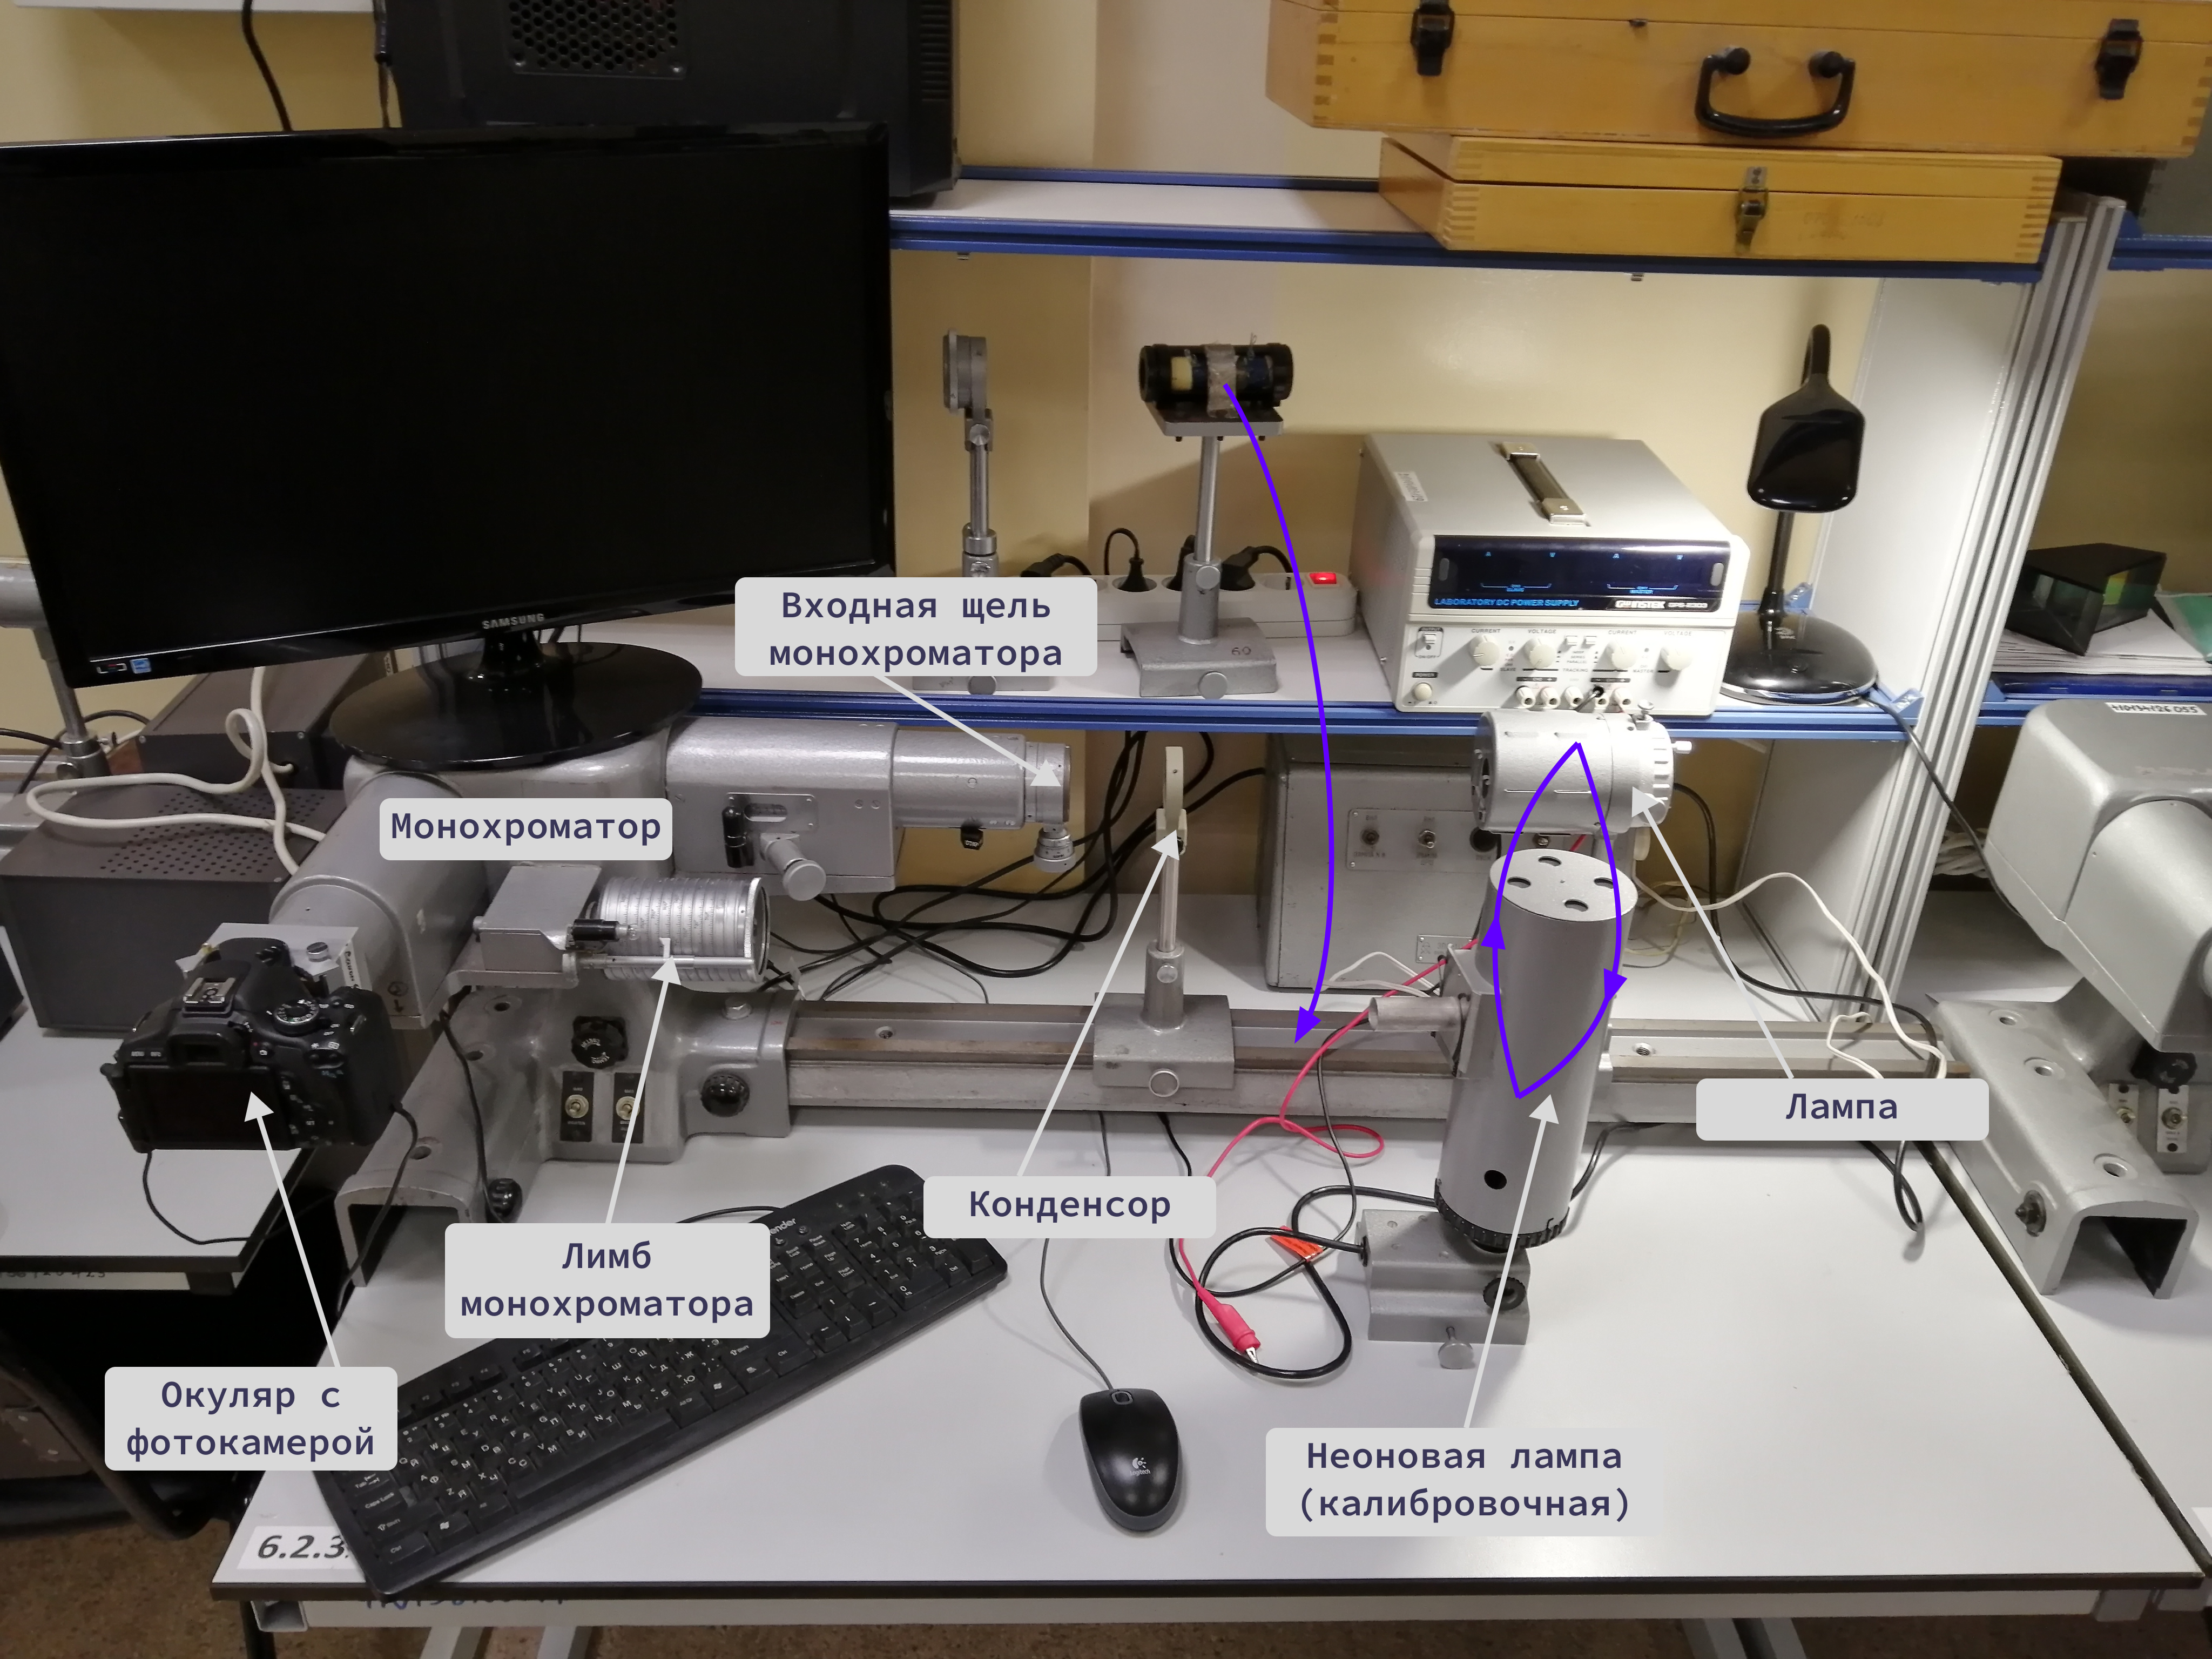
\includegraphics[width=10cm]{res/setup.png}
		
 		\begin{columns}
 			\column{0.35\textwidth}
			\begin{enumerate}
				\item[$\bullet$] L - light source
				\item[$\bullet$] $K$ - condenser
				\item[$\bullet$] $\Phi$ - light filter
				\item[$\bullet$] $O_1, O_2$ - lenses
				\item[$\bullet$] $Q$ - cuvette
				\item[$\bullet$] $M$ - microscope
			\end{enumerate}
			\column{0.70\linewidth}
			\includegraphics[width=6cm]{res/real_setup.png}
		\end{columns}
	\end{frame}

	\begin{frame}
		\frametitle{Phase grating spatial structure observation}
		
				Observation of the spatial structure of the phase grating is complicated. The central problem is that phase grating intensity is \textbf{constant}. Indeed, complex transmittance has the following form:
				$$t(x) = e^{i\varphi(x)},$$ with intensity
				$$I(x) = |f_0(x)|^2 = 1.$$
				
				By the way, there are some methods that allow you to observe the spatial structure.

	\end{frame}

	\begin{frame}
		\frametitle{Dark-field method}
		
		One of the most popular methods is called \textbf{dark-field method}. The idea behind is filtering the central maximum with using the screen, we get:
		
		\begin{equation*}
			\begin{split}
				f_0(x) = e^{i m \cos{\Omega x}} \approx 1 +  i m \cos{\Omega x} \overset{\textbf{filtering}}{=} =  i m \cos{\Omega x}.
			\end{split}
		\end{equation*}
		Then the intensity of the filtered light is the following:
		
		\begin{equation*}
			\begin{split}
				I_f(x) = m^2 \cos{\Omega x}^2 \neq 1.
			\end{split}
		\end{equation*}
	
		Another methods, such as \textbf{phase constrast method}, is based on the transition from a phase grating to an amplitude one.
	\end{frame}

	\begin{frame}
		\frametitle{Phase and Amplitude Grating with Uniform Beam}
		
		\begin{figure}
			\centering
			\includegraphics[width=0.5\linewidth]{res/amplitude_phase_grating}
			\caption{Phase (a) and amplitude (b) grating vector diagrams}
			\label{fig:amplitudephasegrating}
		\end{figure}
		
		The grating modulation functions are respectively ($i$ - matters):
		$$	t(x) = e^{i m \cos \Omega x} \approx 1 + \frac{im}{2}e^{i \Omega x} + \frac{im}{2}e^{-i \Omega x},$$
		
		$$	t(x) = 1 + m \cos{\Omega x} = 1 + \frac{m}{2}e^{i \Omega x} + \frac{m}{2}e^{-i \Omega x}. $$
	
	\end{frame}	

		\begin{frame}
		\frametitle{Shifting the screen}

		In other words, we can see interaction of three waves with the following modulations:
		 $1, \frac{im}{2}e^{i \Omega x},\frac{im}{2}e^{-i \Omega x}$. This gives the following waves equations: 
		$$e^{i kz}, \frac{im}{2}e^{i k(z\cos{\psi} + x\sin{\psi})},\frac{im}{2}e^{i k(z\cos{\psi} - x\sin{\psi})} \; \left(\sin{\psi} = \pm\frac{\Omega}{k}  \right)$$
		
		
		It follows from the above that there is a possibility of the phase-amplitude grating transition. Indeed, let the screen plane shift by $\Delta z$, this will result in the phase shift:
		
		$$\text{Phase shift} = k\Delta z(1 - \cos{\psi}).$$
		
		
		If $\Delta z = \frac{\pi}{2} + 2\pi n$, then the central wave $E_0$ has been rotated by $\frac{\pi}{2}$ and phase-amplitude transition has been occurred.
	\end{frame}

	\begin{frame}
		\frametitle{Results and Discussion}
	\end{frame}

	\begin{frame}
		\frametitle{Acknowlegements}
	\end{frame}
	
	
\end{document}